\chapter{Системийн судалгаа}
\section{Ижил төстэй системүүд}
Уг чиглэлээр гадаадын маш олон системүүд байдаг бөгөөд өргөн сонголт бүхий хэлнүүд, түүнд зориулсан код засварлагч агуулсан байдаг. Одоогоор түгээмэл буй цогц системүүдээс дурьдвал 
\begin{itemize}
  \item Leetcode
  \item Hackerrank
  \item Codeforce
  \item SPOJ
  \item ...
\end{itemize} 
гэх мэт. Эдгээр системүүдийн хэрэглэгчийн код ажиллуулж буй байдал нь нэгэн төрлийн бөгөөд UI/UX-ээрээ голчлон ялгарч байгаа билээ. Хэрэглэгчийн кодыг код засварлагч эсвэл файл уншигчаар хүлээн авч өөрсдийн сервер лүүгээ дамжуулдаг бөгөөд тухайн сервер дээр sandbox\footnotemark{} \footnotetext{хамгаалагдсан хязгаарлагдмал орчин}-д хэрэглэгчийн кодыг stdio\footnotemark{} \footnotetext{Standard input output буюу оролт гаралтын стандарт урсгал}-ийг ихэвчлэн ашиглан шинжилгээ хийж үр дүнг нь буцаан харуулж байна. 

Хэрэглэгчийн оролтоос бусдаар аюулгүй байдал талаас мөн request/submission throttling\footnotemark{} \footnotetext{Хүсэлт болон дамжуулалтын давтамжийг бууруулах}, debouncing\footnotemark{} \footnotetext{Илүүдэл давхар ажиллагааг хязгаарлах} зэрэг стратегиудыг ашигласан байна.  

\clearpage

Монголд хэрэгжүүлсэн болон түгээмэл ашигладаг системүүдээс дурьдвал
\begin{itemize}
  \item SPOJ
  \item Accepted.mn
  \item ...
\end{itemize} зэрэг бодлогын сан, дэд систем байдлаар хэрэгжсэн байна. 

\begin{figure}[h]
  \centering
  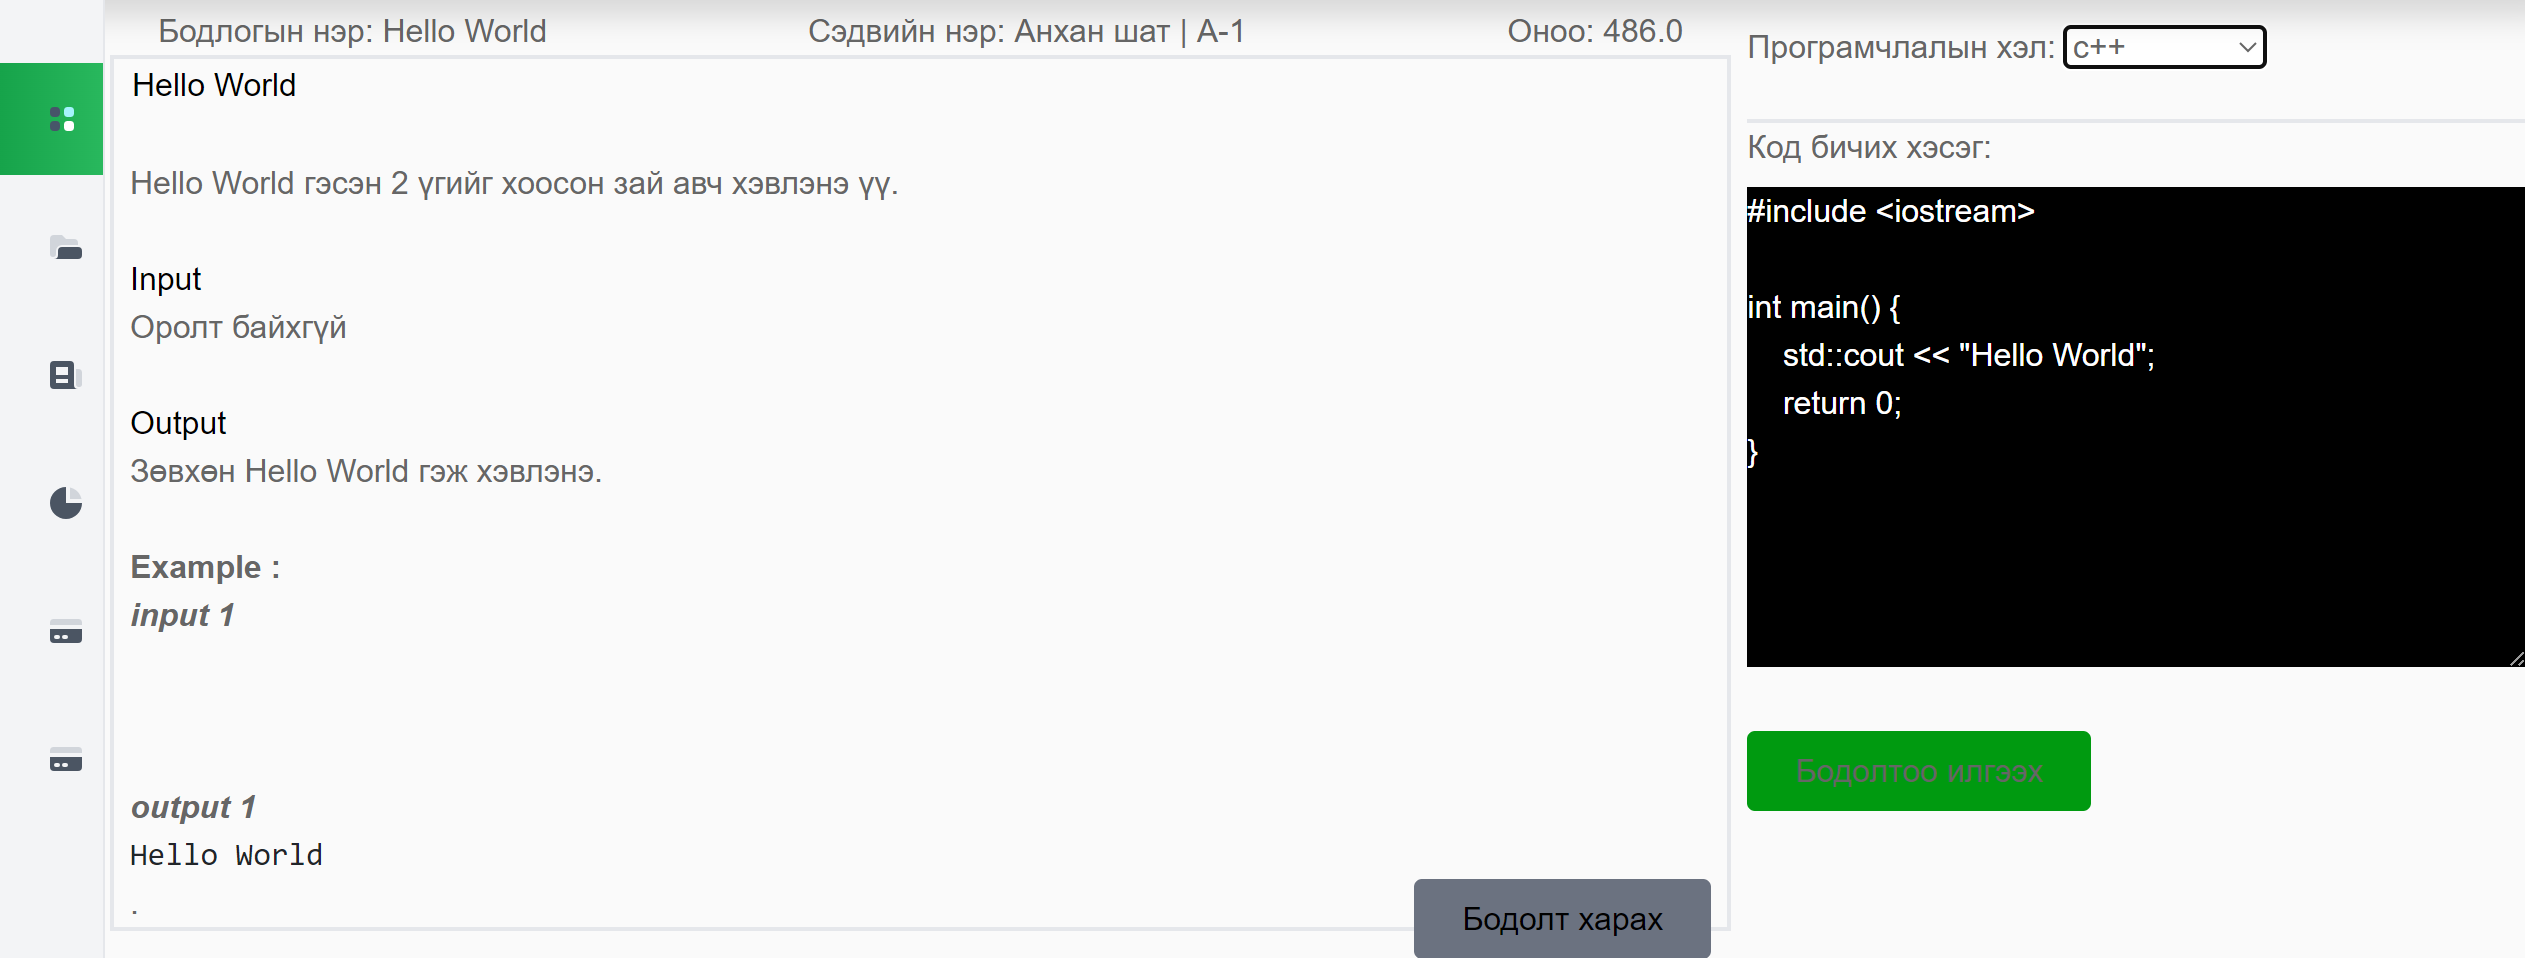
\includegraphics[width=15cm]{img/accepted.PNG}
  \caption{Accepted.mn бодлого бодох}
\end{figure}

\begin{figure}[h]
  \centering
  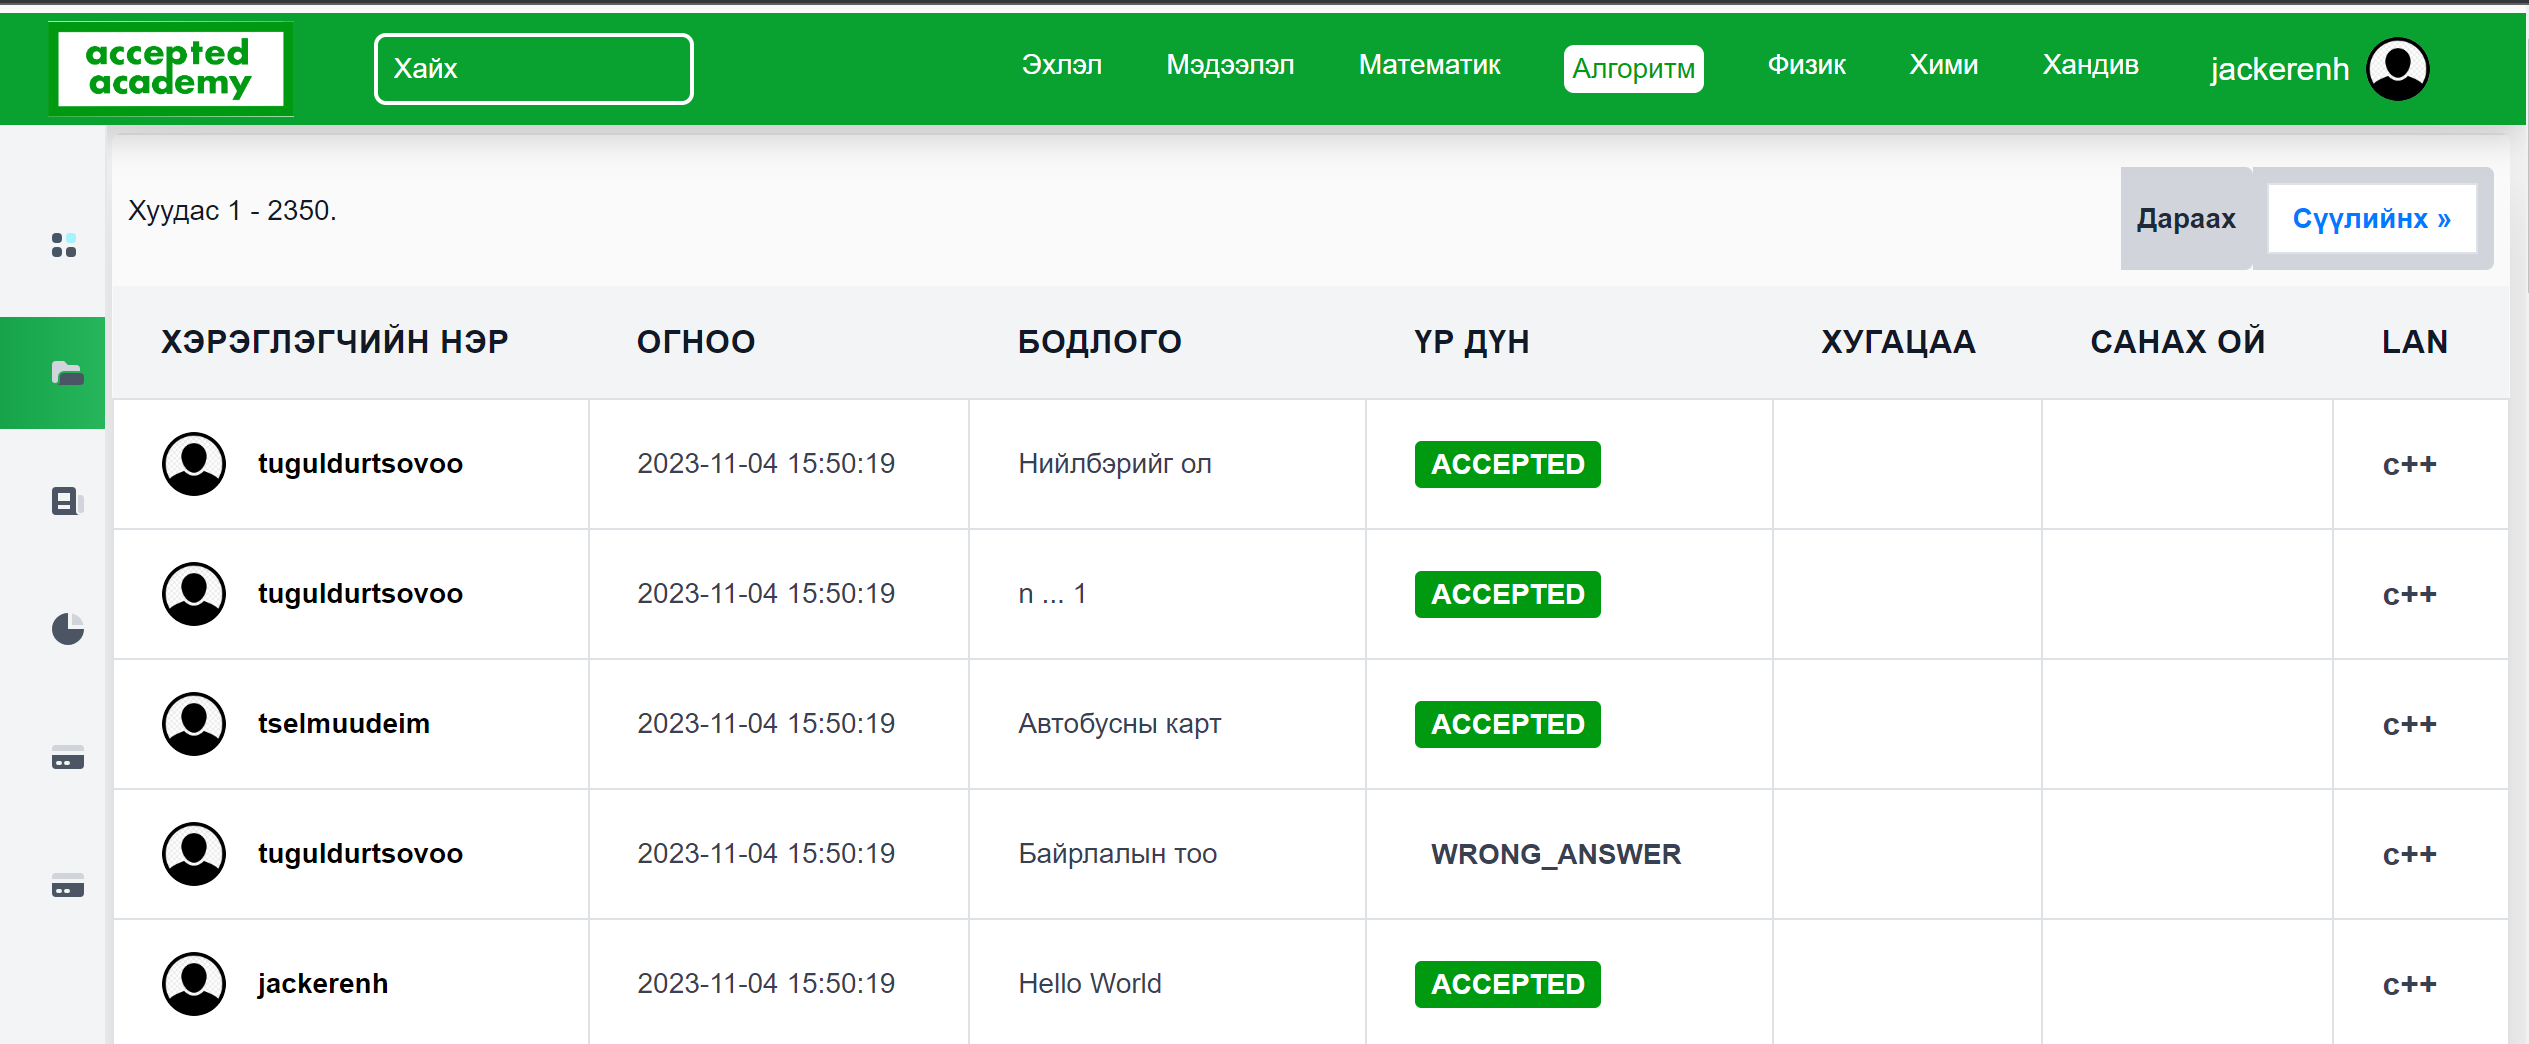
\includegraphics[width=15cm]{img/accepted-judger.PNG}
  \caption{Accepted.mn үр дүн}
\end{figure}

Энэхүү accepted.mn\cite{acceptedmn} нь C/C++, Java, Python, Dart зэрэг програмчлалын хэлнүүдийг дэмждэг сургалтын платформ бөгөөд код засварлагчаар хэрэглэгчийн кодыг хүлээн авч шүүж зөв/буруу статусыг харуулдаг. Тухайн кодыг ажиллуулахдаа websocket технологийг ашиглан сервертэйгээ харьцдаг. One time буюу 1 удаа бичин үр дүнгээ хардаг байдлаар хэрэгжүүлсэн байгаа билээ. 

\begin{figure}[h]
  \centering
  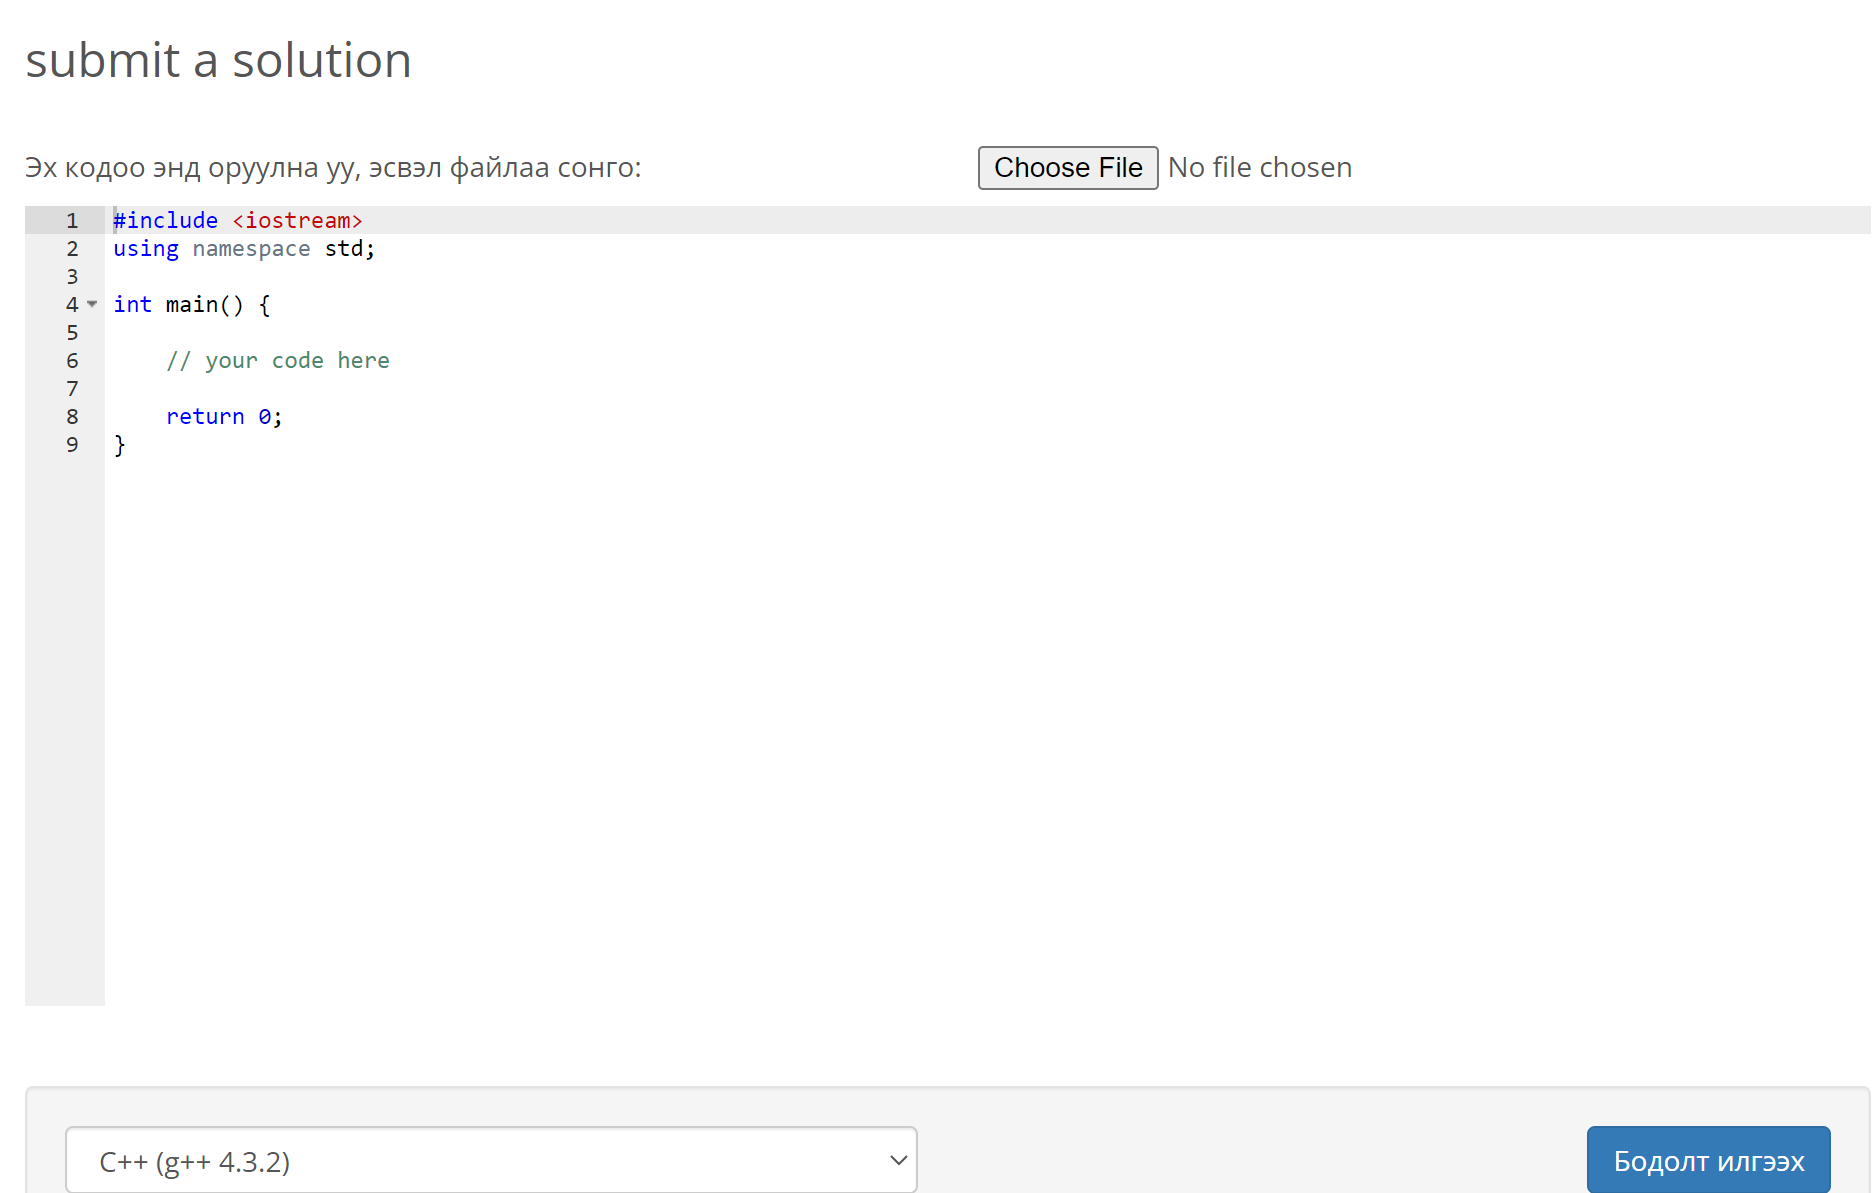
\includegraphics[width=15cm]{img/spoj.PNG}
  \caption{spoj/rgb7 бодлого бодох}
\end{figure}

SPOJ.com\cite{spojmn} нь нийт 41 програмчлалын хэл дэмждэг бөгөөд accepted.mn-ээс ялгаатай нь REST API ашиглан кодыг шүүгч сервер лүү дамжуулдаг. Мөн адил one time байдлаар бичин үр дүнгээ хардаг. 

Эдгээр 2 систем нь тус бүр ижил шинж чанартай тогтмол ашигладаг олон хэрэглэгчтэй бөгөөд хэрэглэгч талдаа тодорхой алдааны мэдээлэл болон хэрэглэгчийн интерфейсийн гүйцэтгэлээрээ гадаадын системүүдээс дутмаг байгааг харж болно. Монгол хэлээр бодлогыг орчуулж оролт гаралтын жишээг тайлбарласан нь зорилтот хэрэглэгчиддээ илүү сайн хүрснийг харж болно. Эдгээр системүүдийг судалсны үндэс дээр хамгийн сайн хэрэгжүүлэлт(Best practice)-үүдийг төлөвлөсөн билээ.

\clearpage

\section{Системийн онцлог}
Програмчлалийн мэдлэгийг нь англи хэл дээр интернет болон нээлттэй сангуудаас хүссэн хүн нь авч болох бөгөөд олон улсын стандарт хэлийг эзэмшсэн байх нь уг салбарын мэргэжилтэнд зайлшгүй байх ёстой чадвар юм. Харин програмчлалд суралцах процесст гадаад хэл болон эх хэл нь өөр нөлөө үзүүлдэг бөгөөд учир шалтгааныг нь бие даан олох, логик сэтгэлгээгээр бодоход эх хэл нь илүү давуу талтайг олон судалгаа баталсан байдаг. Шинжилгээ хийх, логиктой сэтгэх, учир шалтгааныг нь тайлах асуудлууд дээр хийсэн судалгаагаар эх хэл дээрээ суралцсан бүлэг хүмүүс нь илүү сайн үр дүнд хүрдэг болохыг судалж баталсан байдаг\cite{motherLanguage}.

\subsection{Хэрэглэгчийн интерфейс}
Систем нь Монгол хэл бүхий хэрэглэгчийн интерфейстэй байх бөгөөд одоо байгаа ижил төстэй системүүдээс зохиомж болон хэрэглэгчийн интерфейсээрээ ялгарах билээ. Үүнд: 
\begin{itemize}
  \item Intellisense\footnotemark{} \footnotetext{Ухаалаг байдлаар хэрэглэгчид код санал болгогч} бүхий код засварлагч, хэрэглэгчид түүний зарласан функц болон хувьсагчдийг санал болгон код бичих процессийг илүү хялбарчлана.
  \item Хэрэглэгчийн сонголт бүхий код засварлагчийн өнгө, үзэмж, хэрэглэгч өөрийн дассан өнгөний зохицол дээр бичих боломжтой.
  \item Өөрийн бодсон бодлогын бодолт болон бусдын бодолтуудыг харах боломжтой.
  \item Илүү уян хатан програмчлалын хэлний боломжуудыг ашиглах. Үүнд тухайн програмчлалын хэлний built-in өгөгдлийн бүтэц болон бусад сангуудыг ашиглах боломжууд орно. 
  \item Хэрэглэгч өөрийн бичиж буй кодны алдаа тэр дундаа syntax\footnotemark{}-ийн алдааг мөрийн дугаараар илрүүлэх боломжтой. \footnotetext{Код бичиж буй хэрэглэгчээс үүдэлтэй кодны бүтэц, бичиглэлийн алдаа}
  \item Тухайн бодлого нь олон тест кейсээр шалгагдах бөгөөд хэрэглэгч аль тест кейс дээр тэнцээгүйг харуулна.
\end{itemize}

\subsection{Хэрэглэгчийн боломжууд}
Системийн гол зорилго нь эх хэл дээр зөвхөн алгоритм болон кодын логик тал дээр хэрэглэгчийг төвлөрөхөд дэмжих бөгөөд алдааны мэдээлэл болон бусад стандарт програмчлалын ойлголтуудыг англи хэл дээр байлгаж, хэрэглэгчийг тэдгээр нэршлүүдийг судалж, илүү дотно болохыг дэмжинэ.

Хэрэглэгч мөн бодлогоо амжилттай бодсон төлөвт байвал бусдын хэрэгжүүлэлтүүдийг судалж шинжлэх боломжтой болох билээ.

Хэрэглэгчийн ашиглалт талаас дотоодын системүүдээс ялгарч буй зүйлсээс дурьдвал тухайн хэрэглэгч заавал бүртгэл үүсгэлгүйгээр өөрийн бусад платформууд дээр ашигладаг мэдээллээр(Github, Google credentials provider\footnotemark{}\footnotetext{Хэрэглэгчийн мэдээллийг зөвшөөрлийн дагуу олгох платформууд}) нэвтэрч орон тэгш эрхтэйгээр ашиглах боломжтой. Мөн хэрэглэгч 1 time буюу тухайн бодолтоо submission хийх процесс руу дамжуулаад үр дүнгээ хүлээхийн оронд тухайн бодолтоо илүү бодит үр дүнтэйгээр тухайн хуудсан дээр засвар оруулан дахин оролдлого хийх боломжтой. Одоогийн дотоодод ашиглаж буй системүүд нь алдааны тодорхой мэдээлэл дутмаг, мөн хэрэглэгчийн үр дүнг гаргахын тулд тухайн хэрэглэгчийн дараа дараачийн submission процессуудыг хуудас шилжин, төлөвт оруулан шинжилдэг. Энэхүү процессийг "Coldbrains" системээр хэрэглэгч талдаа илүү ойлгомжтой,тодорхой болгож шийдсэн бөгөөд хэрэглэгч удаа дараа тухайн кодыг хүлээж автал олон оролдлого 1 дор хийх боломжуудыг бий болгож байгаа билээ.
